\documentclass[compress]{beamer}
\usepackage{ifthen,verbatim}

\newcommand{\isnote}{}
\xdefinecolor{lightyellow}{rgb}{1.,1.,0.25}
\xdefinecolor{darkblue}{rgb}{0.1,0.1,0.7}

%% Uncomment this to get annotations
%% \def\notes{\addtocounter{page}{-1}
%%            \renewcommand{\isnote}{*}
%% 	   \beamertemplateshadingbackground{lightyellow}{white}
%%            \begin{frame}
%%            \frametitle{Notes for the previous page (page \insertpagenumber)}
%%            \itemize}
%% \def\endnotes{\enditemize
%% 	      \end{frame}
%%               \beamertemplateshadingbackground{white}{white}
%%               \renewcommand{\isnote}{}}

%% Uncomment this to not get annotations
\def\notes{\comment}
\def\endnotes{\endcomment}

\setbeamertemplate{navigation symbols}{}
\setbeamertemplate{headline}{\mbox{ } \hfill
\begin{minipage}{5.5 cm}
\vspace{-0.75 cm} \small
\end{minipage} \hfill
\begin{minipage}{4.5 cm}
\vspace{-0.75 cm} \small
\begin{flushright}
\ifthenelse{\equal{\insertpagenumber}{1}}{}{Jim Pivarski \hspace{0.2 cm} \insertpagenumber\isnote/\pageref{numpages}}
\end{flushright}
\end{minipage}\mbox{\hspace{0.2 cm}}\includegraphics[height=1 cm]{../cmslogo} \hspace{0.1 cm} \includegraphics[height=1 cm]{../tamulogo} \hspace{0.01 cm} \vspace{-1.05 cm}}

\begin{document}
\begin{frame}
\vfill
\begin{center}
\textcolor{darkblue}{\Large CSC Beam-Halo Alignment}

\vfill
\begin{columns}
\column{0.3\linewidth}
\begin{center}
\large
\textcolor{darkblue}{\it Jim Pivarski}

Aysen Tatarinov

Vadim Khotilovich

Alexei Safonov
\end{center}
\end{columns}

\begin{columns}
\column{0.3\linewidth}
\begin{center}
\scriptsize
{\it Texas A\&M University}
\end{center}
\end{columns}

\vfill
 7 May, 2010

\end{center}
\end{frame}

%% \begin{notes}
%% \item This is the annotated version of my talk.
%% \item If you want the version that I am presenting, download the one
%% labeled ``slides'' on Indico (or just ignore these yellow pages).
%% \item The annotated version is provided for extra detail and a written
%% record of comments that I intend to make orally.
%% \item Yellow notes refer to the content on the {\it previous} page.
%% \item All other slides are identical for the two versions.
%% \end{notes}

\small

\begin{frame}
\frametitle{Outline}
\begin{itemize}\setlength{\itemsep}{0.5 cm}
\item Method to align all rings, not just complete ones

\item Ring-radius corrections

\item New constants

\item Error analysis
\end{itemize}
%% \hspace{-0.83 cm} \textcolor{darkblue}{\Large Outline2}
\end{frame}

\begin{frame}
\frametitle{Reminder}

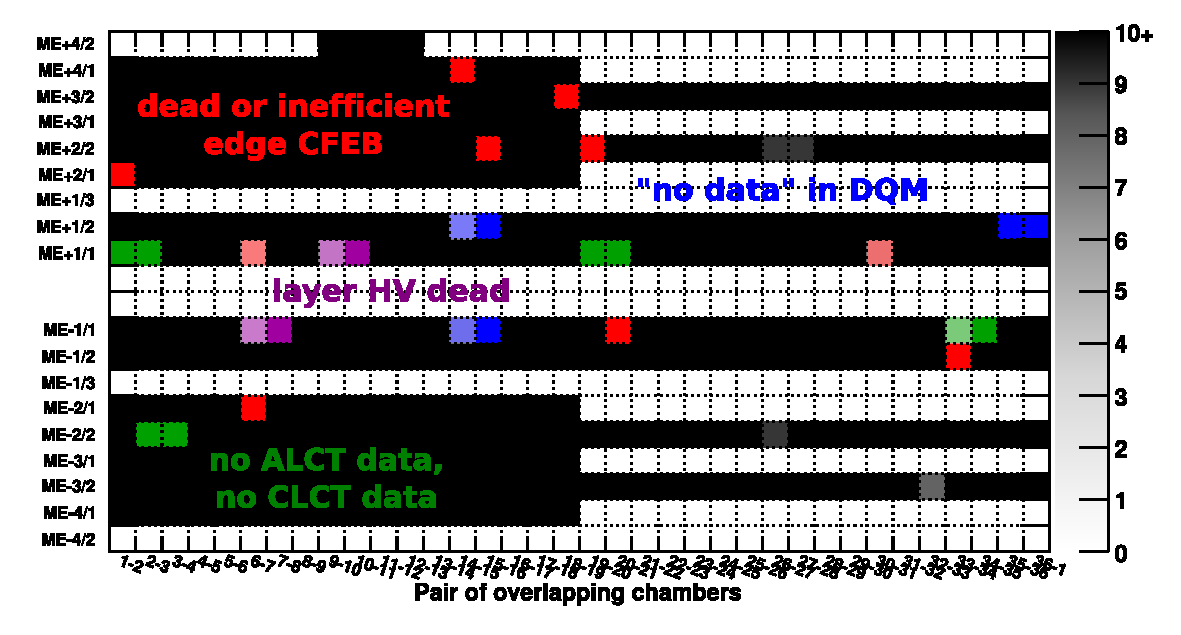
\includegraphics[width=\linewidth]{occupancy_problems.pdf}

\begin{itemize}
\item We can't rely on reading out data from all CSC edges
\item Old procedure relied on complete rings for a full set of equations
\item That left only 4 alignable rings--- not acceptable
\end{itemize}
\end{frame}

\begin{frame}
\frametitle{Mathematical framework}

\begin{columns}
\column{0.5\linewidth}
\vspace{0.5 cm}
\only<1>{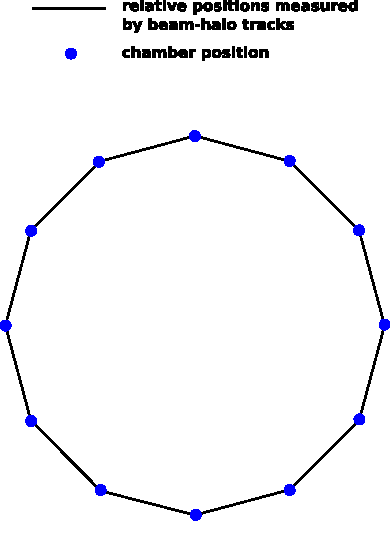
\includegraphics[width=\linewidth]{beamhalo0.pdf}}
\only<2>{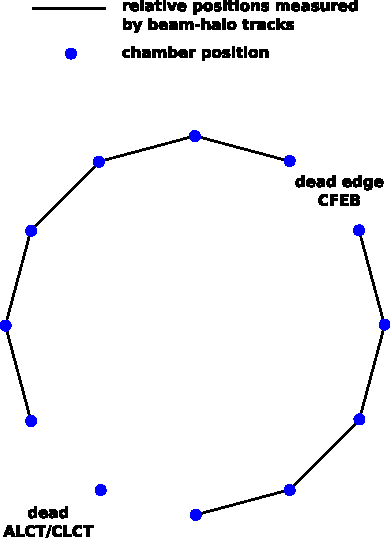
\includegraphics[width=\linewidth]{beamhalo.pdf}}
\only<3>{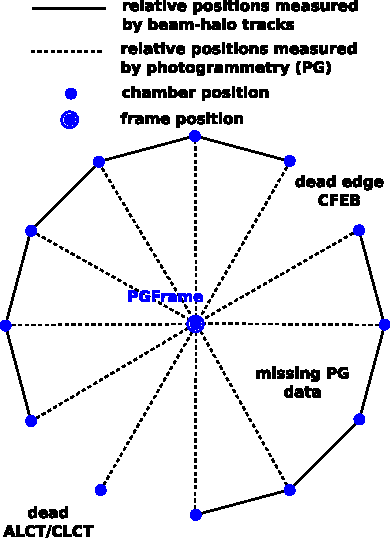
\includegraphics[width=\linewidth]{beamhalo-PG.pdf}}
\only<4>{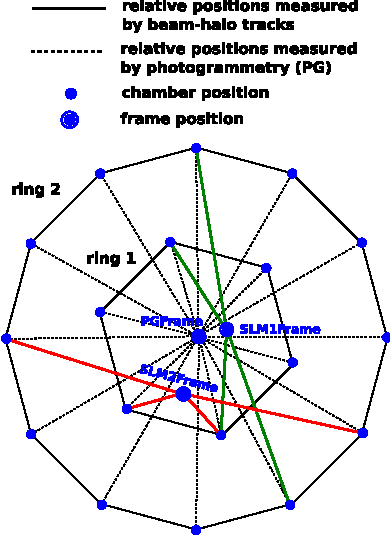
\includegraphics[width=\linewidth]{beamhalo-PG-SLM.pdf}}

\column{0.5\linewidth}
\only<1>{\begin{itemize}
\item Residuals relate chambers $i$ and $i+1$: for $N$ chambers,
  that's $N$ equations
\item Rotation angle of whole ring cannot be determined, so really only
  $N-1$ independent equations
\item Last constraint is closure:

\mbox{ } \hfill $\displaystyle \frac{1}{N}\sum_{i}^{N} r_i$ should be zero \hfill \mbox{ }
\end{itemize}}
\only<2>{\begin{itemize}
\item If one constraint is missing, we could fill in the information
  by {\it assuming} closure

\item Problem: closure became non-zero when the field was turned on
  (will revisit later in this talk)

\item Another problem: many rings had more than one missing
  constraint--- system is underdetermined

\item However, in complete rings we find that photogrammetry (PG) is still
  accurate: can use PG as a new constraint
\end{itemize}}
\only<3-4>{\begin{itemize}
\item New framework to combine beam-halo and PG on an
  equal footing:
\begin{itemize}
\item generalize equations to relate any $i$ and $j$
\item PG measurements relate each chamber $i$ with an external frame,
  a new chamber-like object
\end{itemize}
\item Even with gaps in beam-halo and PG, the system is always
  constrained or overconstrained (graph is fully connected)
\item<4> Potential extension (not in this talk): SLMs also relate
  groups of chambers to frames; I made new software flexible enough to
  possibly include it
\end{itemize}}
\end{columns}
\end{frame}

\begin{frame}
\frametitle{Radius corrections}

\begin{itemize}
\item Closure constraint in 2008 $\vec{B}=0$ data uncovered detector \mbox{width issue\hspace{-1 cm}}
\item Shape of individual chambers has not changed \mbox{(in reality and software)\hspace{-1 cm}}
\item New data with full $\vec{B}$ has non-zero closure, independent \mbox{of momentum\hspace{-1 cm}}
\item Non-zero closure is equivalent to either incorrect detector widths {\it or} incorrect ring radius
\item Disk bending {\it does} change ring radius, since chamber
  centers are displaced in $z$ from the disk: rotation is around a
  point outside the chamber
\end{itemize}

\vspace{-0.5 cm}
\mbox{ } \hfill 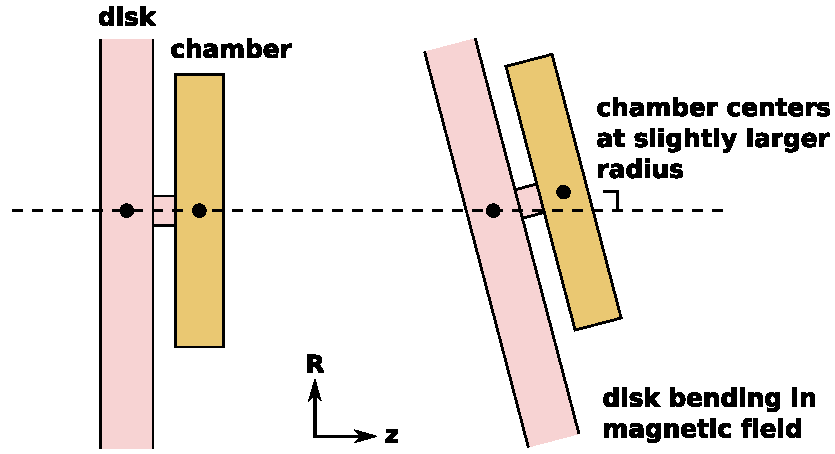
\includegraphics[width=0.6\linewidth]{olegs_correction.pdf} \hfill \mbox{ }
\end{frame}

\begin{frame}
\frametitle{Radius corrections}

\begin{itemize}
\item Oleg did a back-of-the-envelope calculation and predicted that
  including this effect would account for half of the observed discrepancy
\item Putting these numbers into the full reconstruction (accounting
  for the fact that even- and odd-numbered chambers have different
  length posts) yields Oleg's prediction
\end{itemize}

\begin{center}
\renewcommand{\arraystretch}{1.3}
\begin{tabular}{c c c c}
\hline\hline
& 2008 (no $\vec{B}$) & 2010 (full $\vec{B}$) & corrected 2010 \\\hline
ME$+$3/1 &                       & $+$298~mm & $+$100 $\pm$ 9~$\mu$m \\
ME$-$2/1 & $-$40 $\pm$ 23~$\mu$m & & \\
ME$-$3/1 & $-$20 $\pm$ 28~$\mu$m & $+$486~mm & $+$278 $\pm$ 9~$\mu$m \\
ME$-$3/2 &                       & $+$572~mm & $+$446 $\pm$ 27~$\mu$m \\
ME$-$4/1 &                       & $+$440~mm & $+$267 $\pm$ 10~$\mu$m \\\hline\hline
\end{tabular}
\end{center}
\end{frame}

\begin{frame}
\frametitle{Radius corrections}

\begin{itemize}
\item We can calculate approximate closure of incomplete rings by averaging the residuals we do see:

\mbox{ } \hfill $c = \displaystyle \frac{1}{N_{\mbox{\scriptsize visible}}}\sum_{i}^{N_{\mbox{\scriptsize visible}}} r_i \approx \frac{1}{N}\sum_{i}^{N} r_i$ \hfill $\displaystyle \Delta\mbox{radius} = \frac{c \times N}{2\pi}$ \hfill \mbox{ }

\item Pattern has a compelling symmetry/antisymmetry: strongly suggests a real effect (for which we don't have a complete model)
\end{itemize}

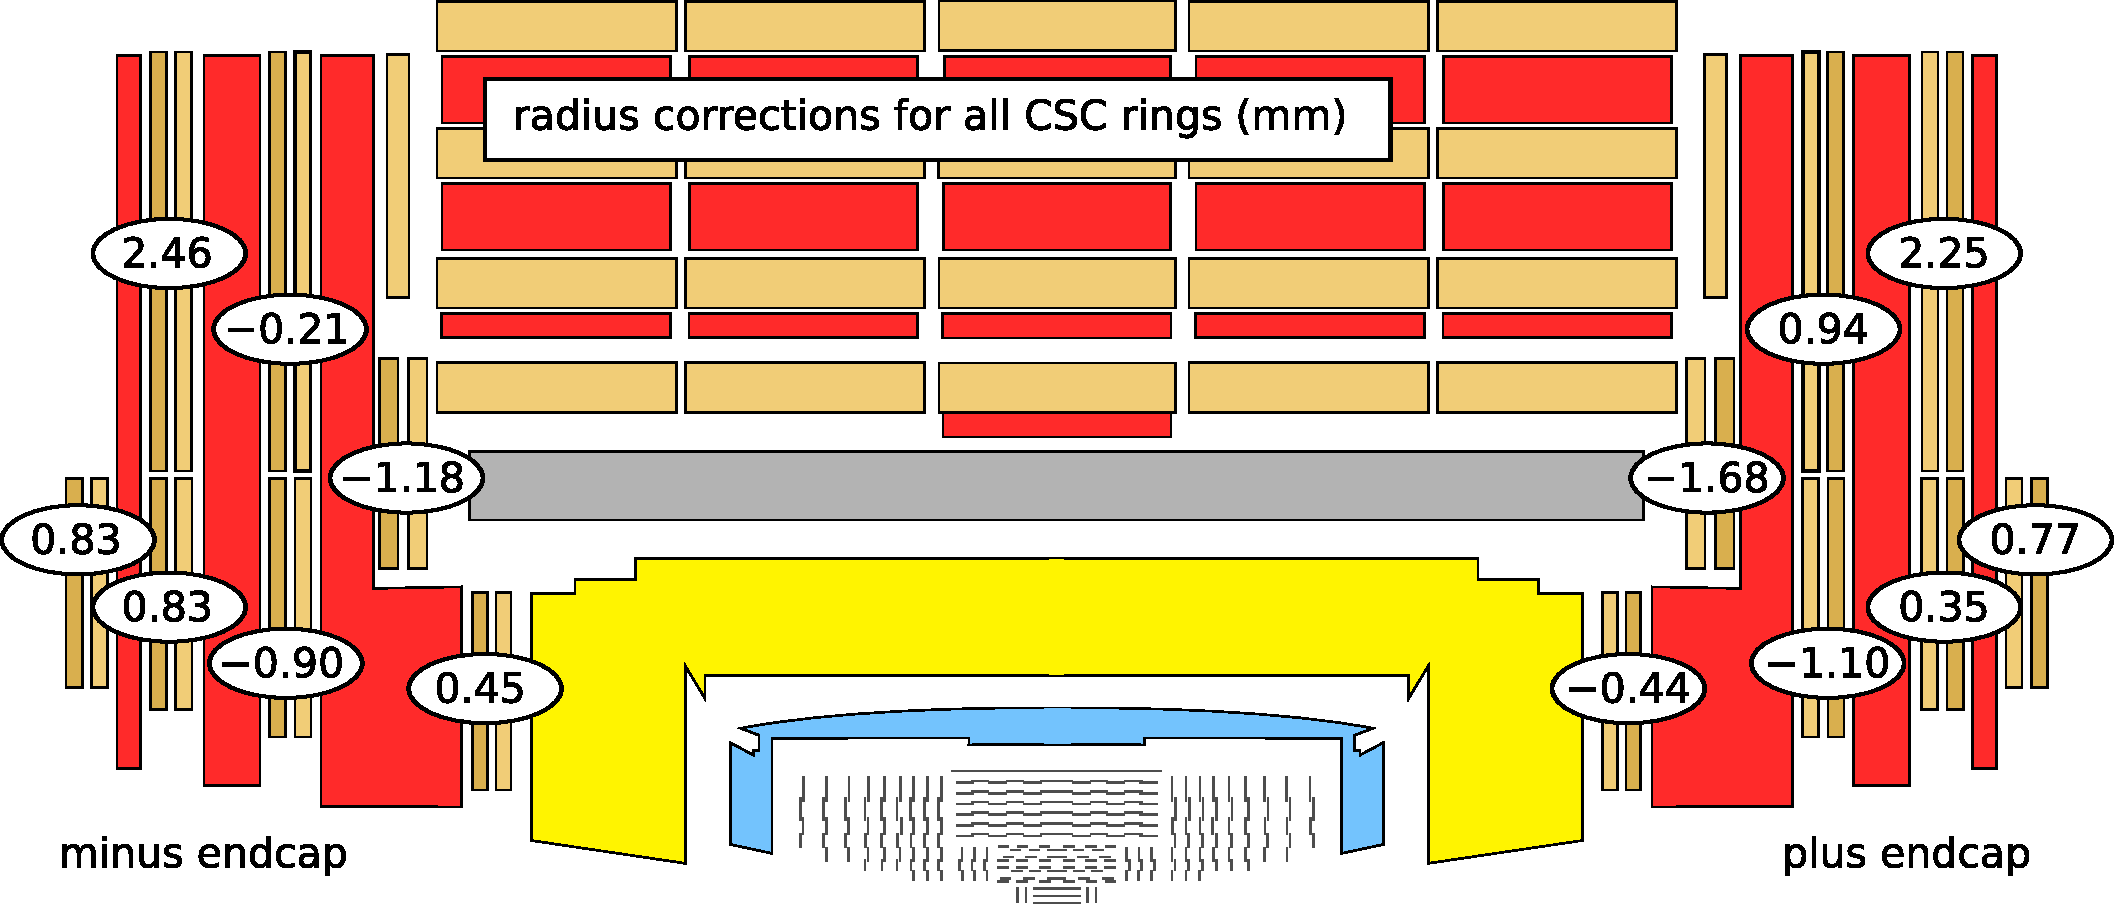
\includegraphics[width=\linewidth]{radial_corrections.pdf}
\end{frame}

\begin{frame}
\frametitle{New constants}

\begin{itemize}
\item If we apply the observed closures as {\it measurements} of ring
  radii, we can move on to align $r\phi$ and $\phi_z$ of all CSCs
  (except ME1/3)

\item Let's look at some of the $r\phi$ alignment results, given the new radii

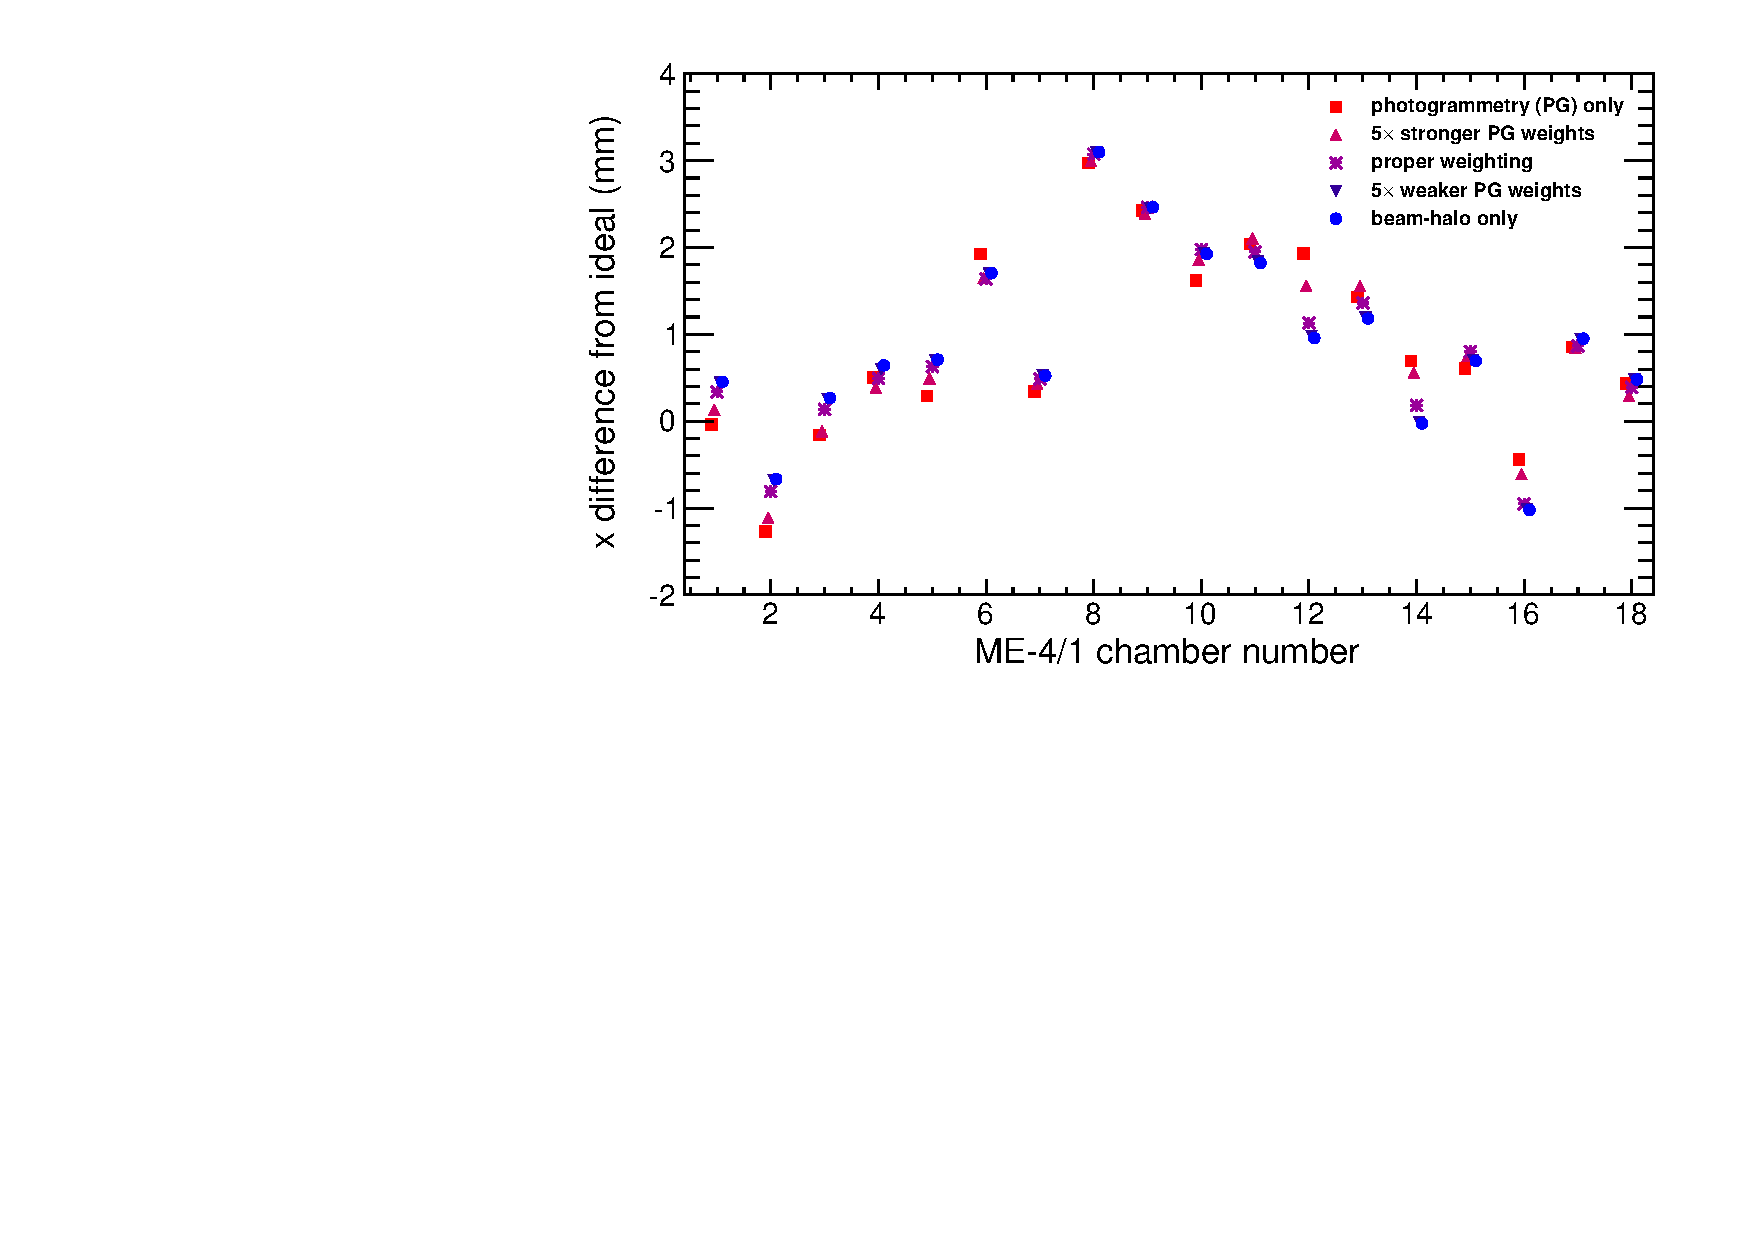
\includegraphics[width=\linewidth]{dependence_on_weights_41.pdf}

\item Pure PG is not very far from pure beam-halo, but now we can
  align them in a combined fit (demonstrated by varying weights)
\end{itemize}
\end{frame}

\begin{frame}
\frametitle{New constants}

\begin{itemize}
\item Another example: this ring has incomplete PG
\item Pure PG has no information about this chamber (set to ideal),
  but even strongly-weighted PG yields a reasonable value for the missing
  chamber because it is ``filled in'' by beam-halo data
\end{itemize}

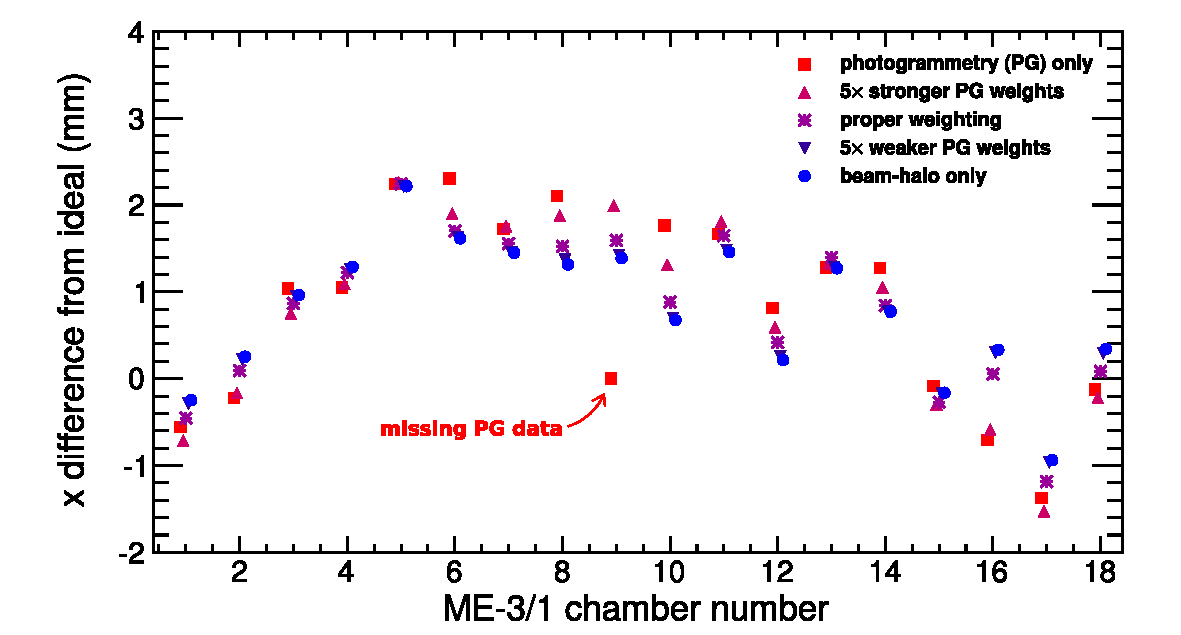
\includegraphics[width=\linewidth]{dependence_on_weights_31.pdf}
\end{frame}

\begin{frame}
\frametitle{New constants}

\begin{itemize}
\item This ring has incomplete beam-halo; system of equations cannot
  be solved without external information
\item Even weakly-weighted PG yields a reasonable value for the
  missing overlap
\end{itemize}

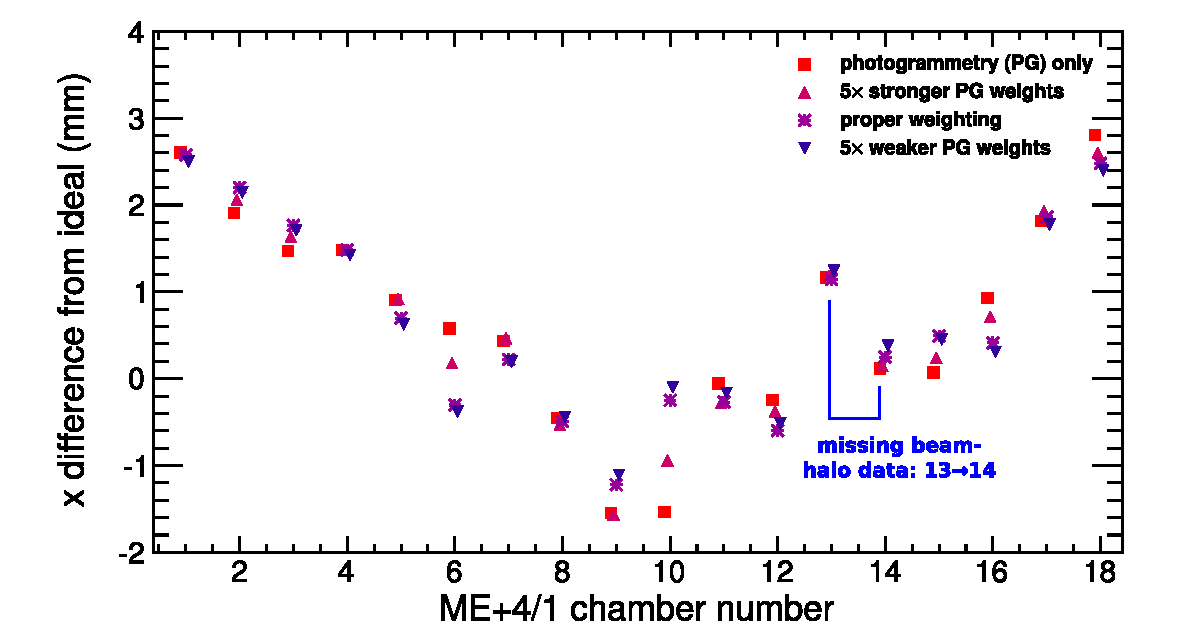
\includegraphics[width=\linewidth]{dependence_on_weights_p41.pdf}
\end{frame}

\begin{frame}
\frametitle{New constants}

\begin{itemize}
\item An outer ring (low beam-halo statistics) with several missing
  chambers in a row: the relative positions of these are entirely
  determined by PG
\end{itemize}

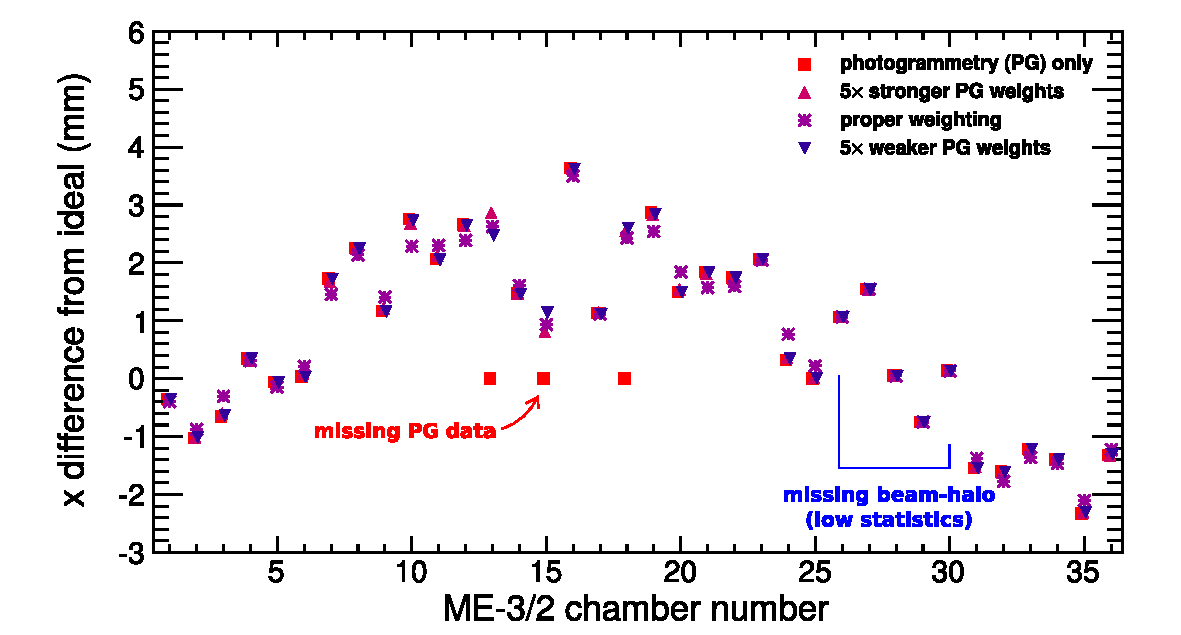
\includegraphics[width=\linewidth]{dependence_on_weights_32.pdf}
\end{frame}

\begin{frame}
\frametitle{New constants}

\begin{itemize}
\item Also works for $\phi_z$ rotation angle

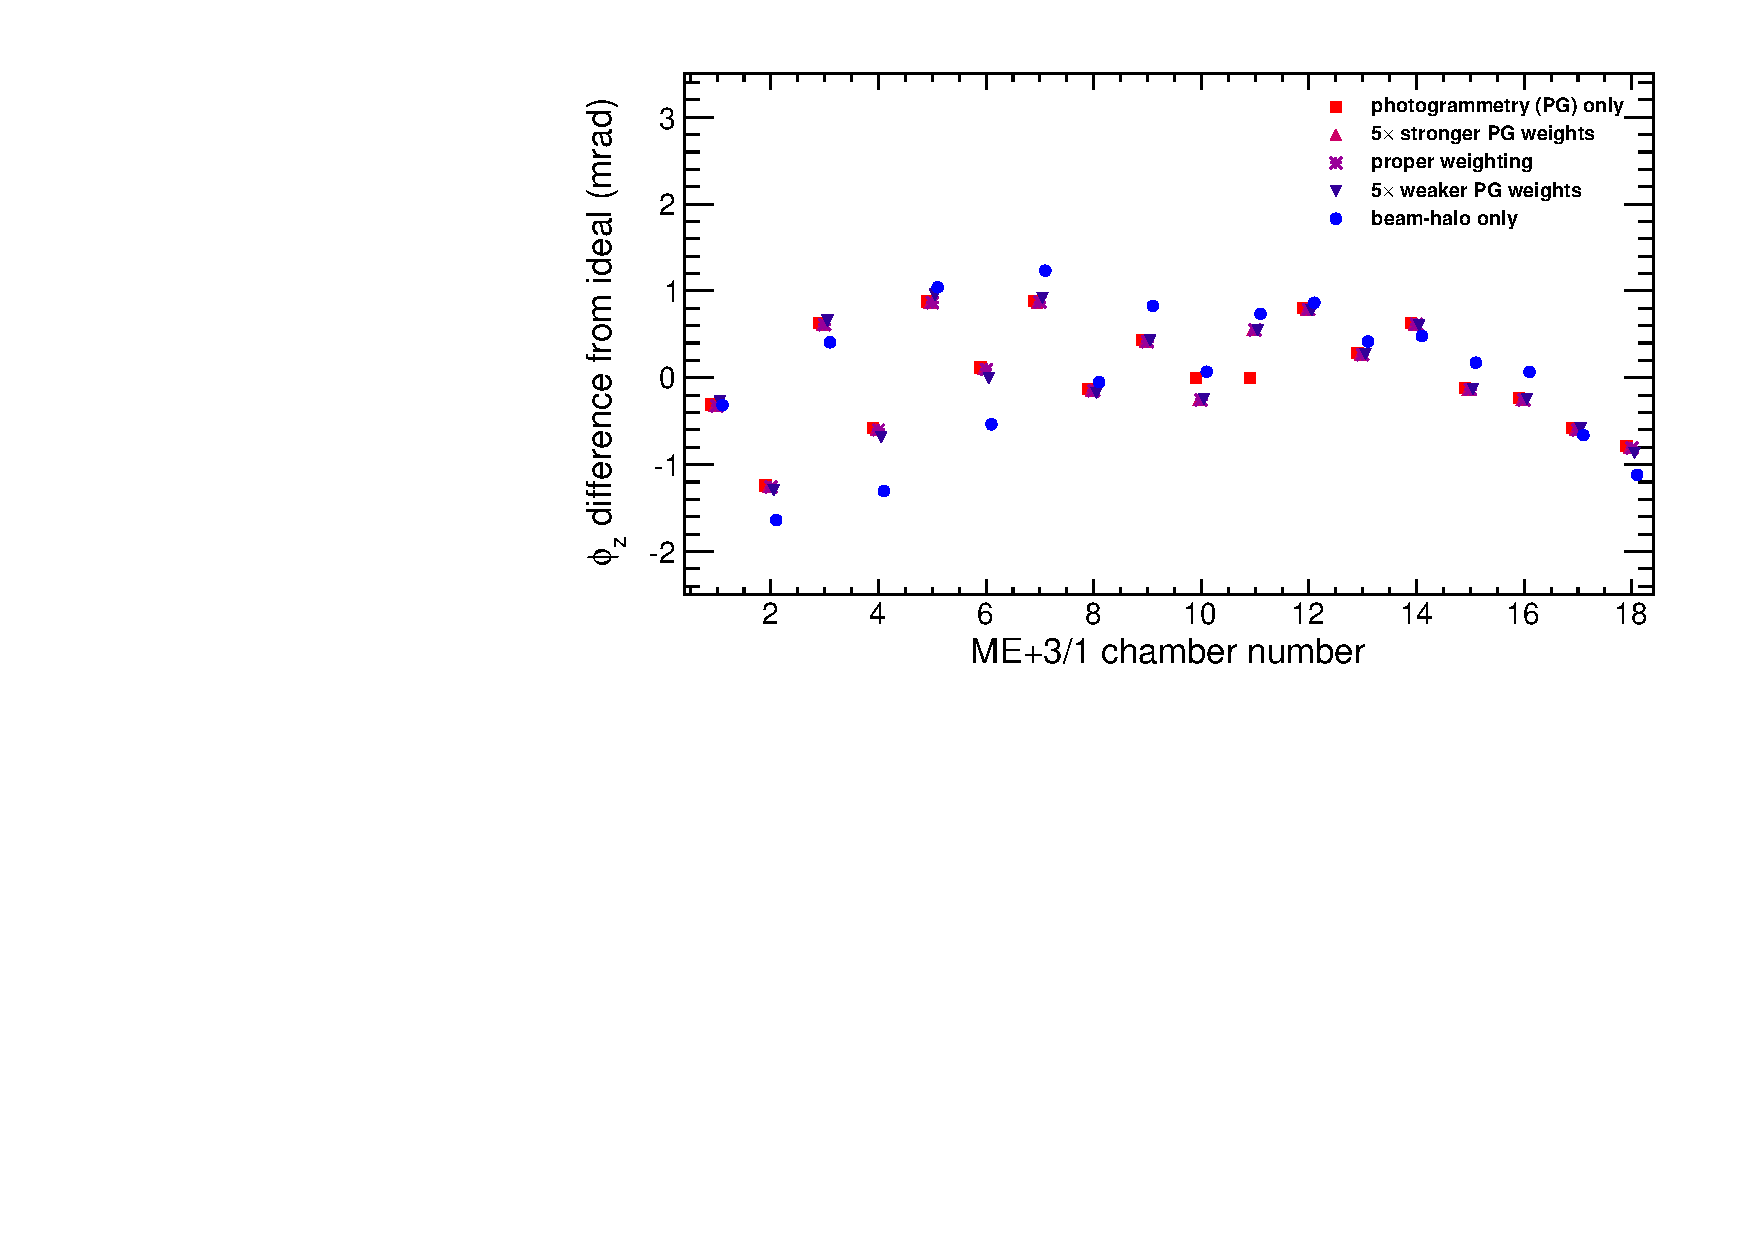
\includegraphics[width=\linewidth]{dependence_on_weights_p31phiz.pdf}

\item Two alignment parameters, $r\phi$ and $\phi_z$, in addition to ring radii
\begin{itemize}
\item third possible parameter, $\phi_y$, is imprecise when measured
  with beam-halo (ideal geometry is more accurate, so leave as ideal)
\end{itemize}
\end{itemize}
\end{frame}

\begin{frame}
\frametitle{New constants}

\begin{itemize}
\item ME1/1 is a special case: no PG constraints available, and some
  chambers are missing (alignment graph is not fully connected)
\end{itemize}

\begin{columns}
\column{0.7\linewidth}
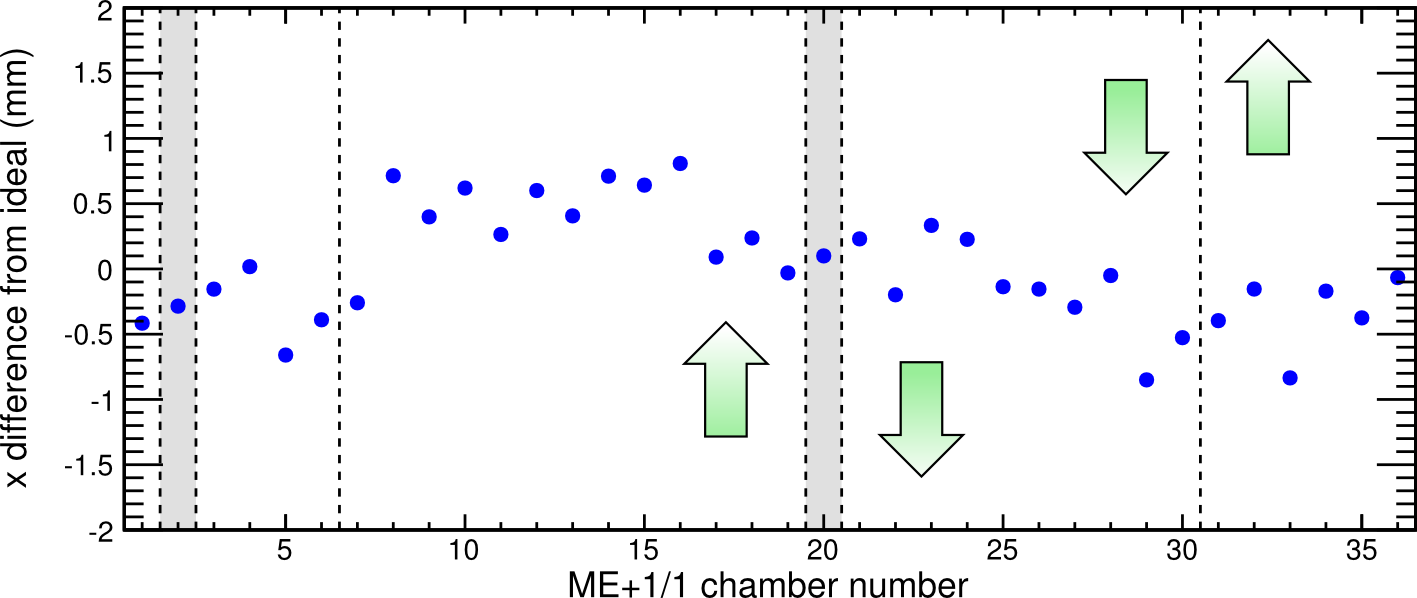
\includegraphics[width=\linewidth]{dependence_on_weights_p11.png}

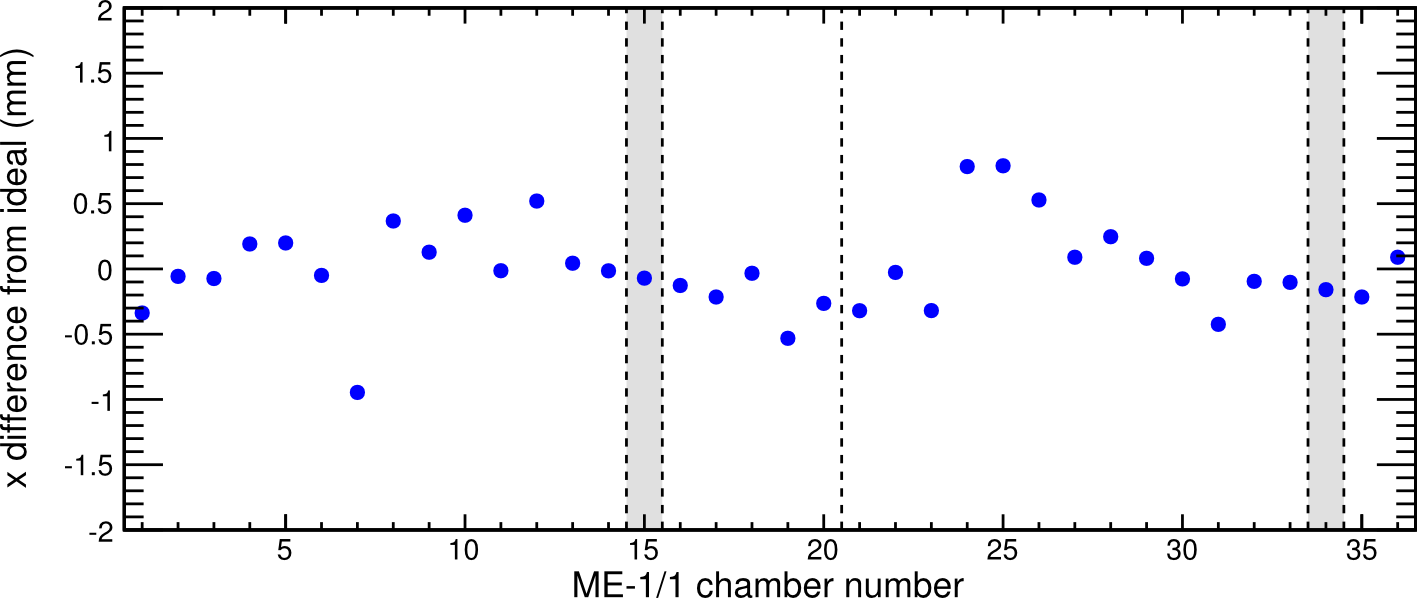
\includegraphics[width=\linewidth]{dependence_on_weights_m11.png}

\column{0.35\linewidth}
\begin{itemize}
\item Dashed lines indicate missing connections

\item We can align the disconnected sections, but these sections will
  later need to be positioned relative to the tracker using
  globalMuons

\item ME1/1 geometry is very nearly ideal
\end{itemize}
\end{columns}
\end{frame}

\begin{frame}
\frametitle{Error analysis}

\begin{itemize}\setlength{\itemsep}{0.25 cm}
\item What is the uncertainty in chamber positions?
\item \ldots a complicated question because chamber uncertainties are highly
  correlated by the system of equations
\item However, the equations can be represented as a matrix, and that
  matrix can be diagonalized to identify a basis of
  linearly-independent combinations of alignment parameters
\item These are ``modes'': modes with small uncertainties are strong
  modes, modes with large uncertanties are {\it weak modes}
\item There are as many modes as there are chambers in the alignment
\end{itemize}
\end{frame}

\begin{frame}
\frametitle{Error analysis}

\begin{itemize}
\item \only<1>{Uncertainty in each mode (mm) for ME+4/1 with a plot of the mode as
  normalized eigenfunction versus chamber number}\only<2>{Uncertainty in each mode (mm) for ME+4/1, this time wtih PG constraint: ``PGFrame'' is last point, right edge of plot window}

\only<1>{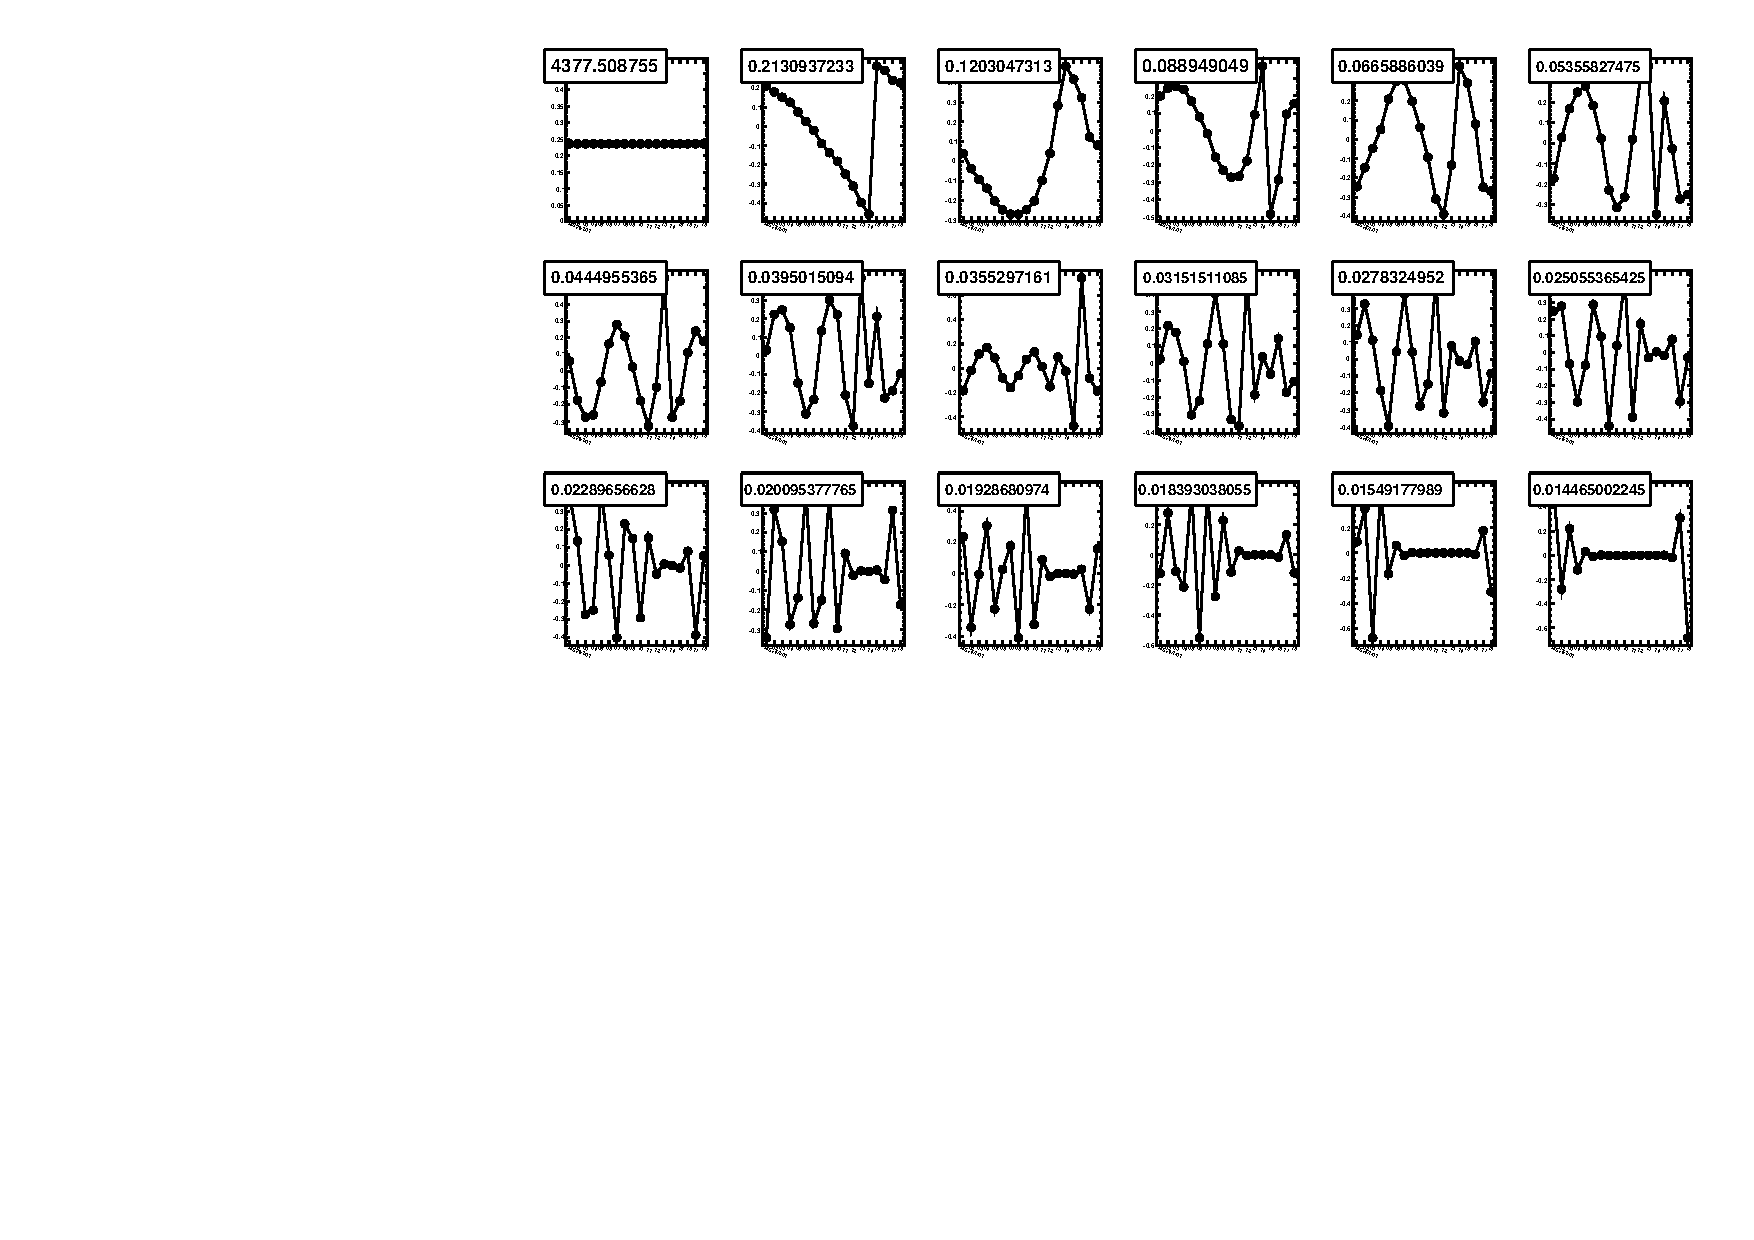
\includegraphics[width=\linewidth]{errormodes_purebh_p41.pdf}}
\only<2>{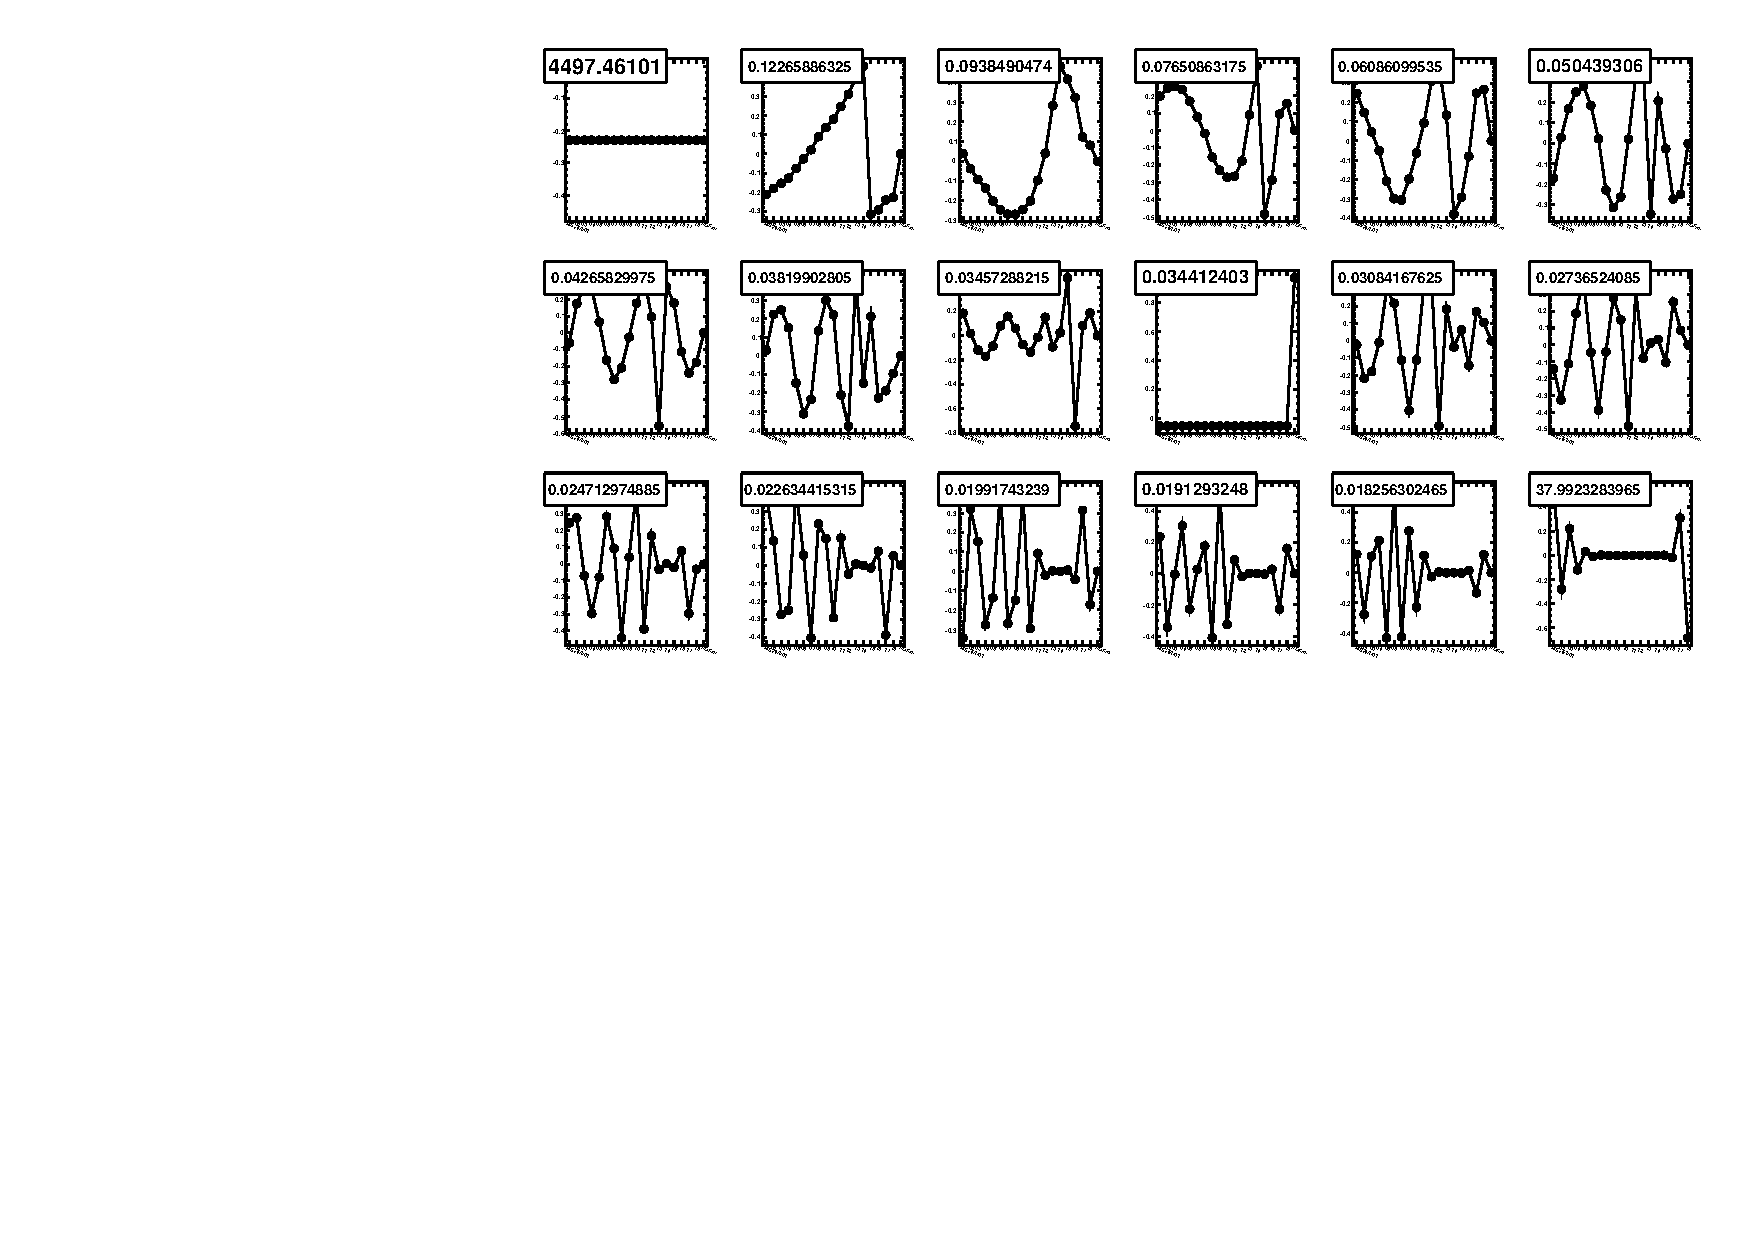
\includegraphics[width=\linewidth]{errormodes_pgnormal_p41.pdf}}

\item<1>{First mode is uncertainty in the position of the whole ring,
  proportional to an arbitrary constant $\lambda$ (set to a large number)}
\item<1> Whole ring position (relative to tracker) requires \mbox{external globalMuons\hspace{-1 cm}}
\end{itemize}
\end{frame}

\begin{frame}
\frametitle{Error analysis}

\begin{itemize}
\item A bigger example: ME+2/2
\item The largest meaningful uncertainty is 0.26 mm
\end{itemize}

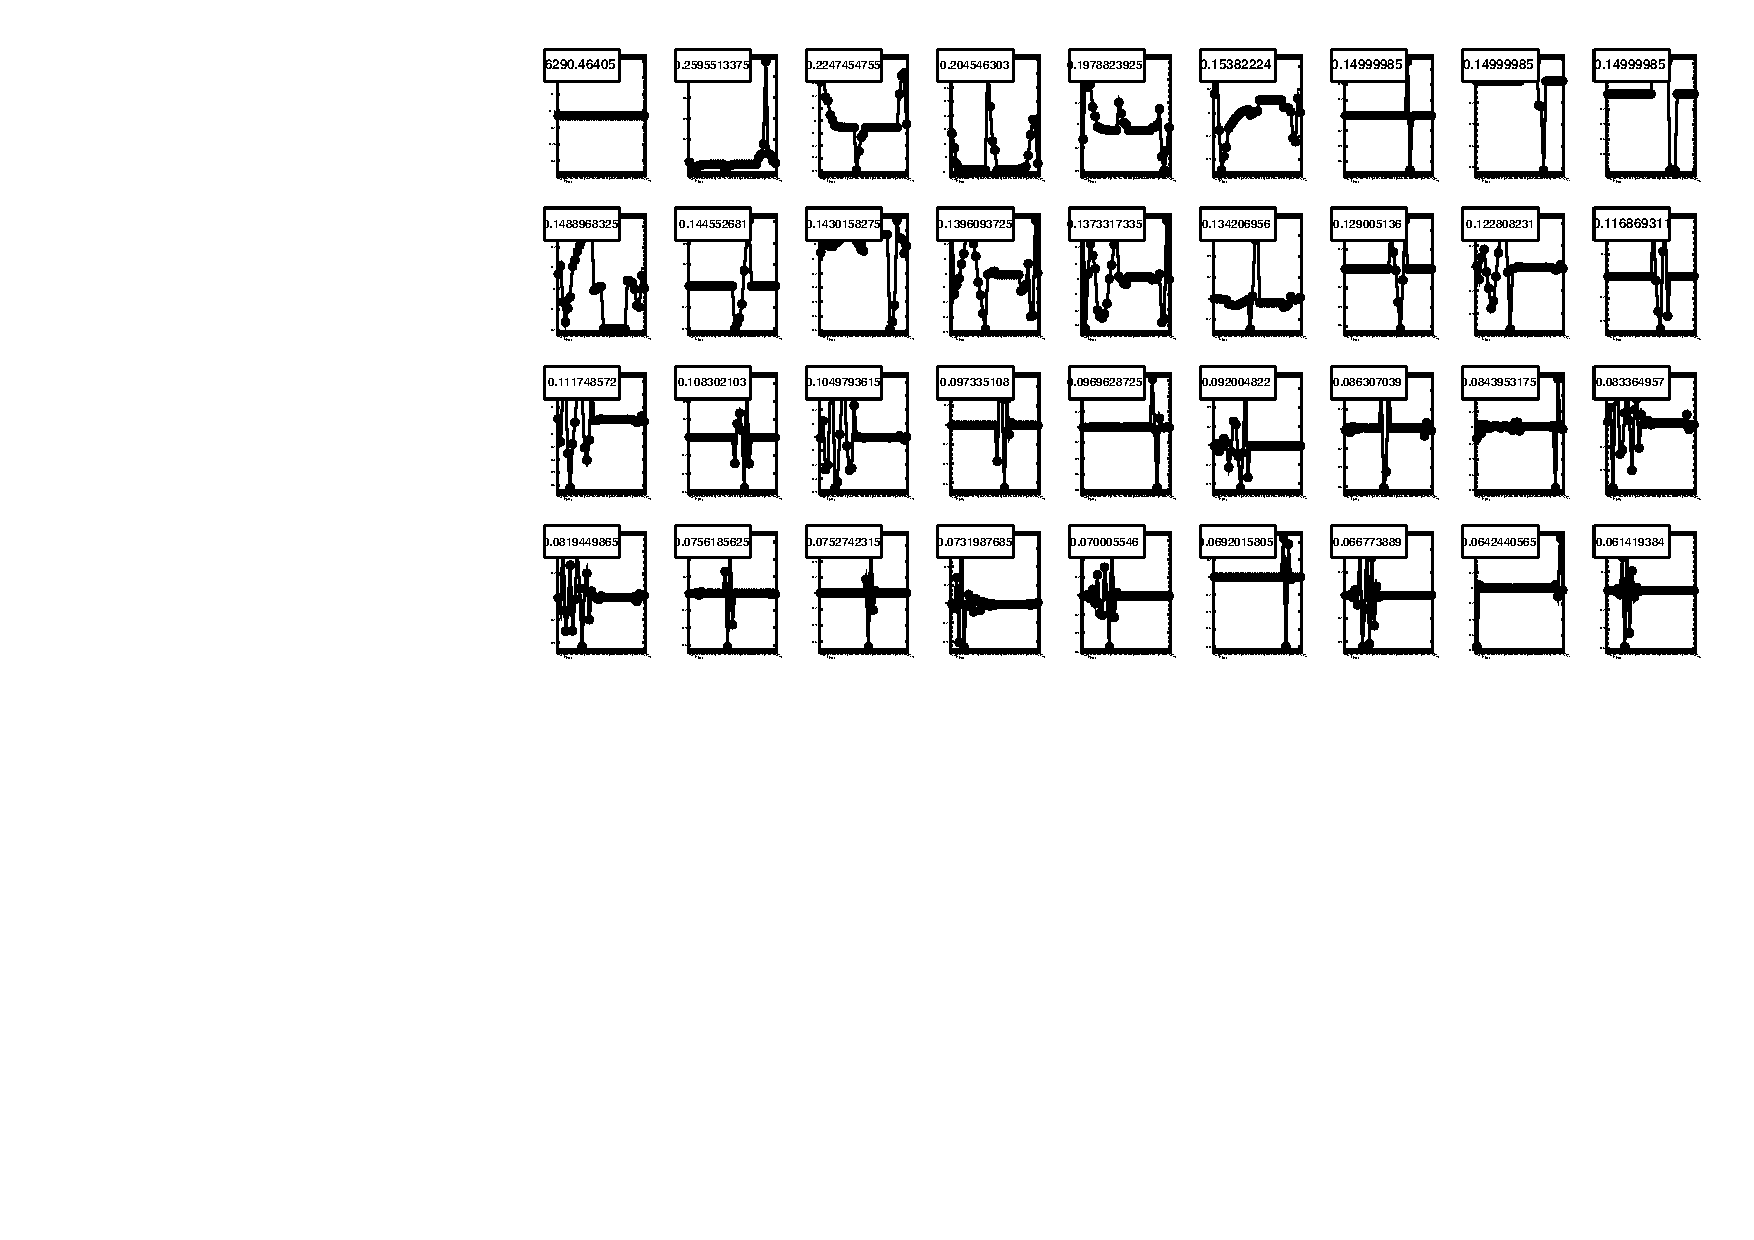
\includegraphics[width=\linewidth]{errormodes_pgnormal_p22.pdf}
\end{frame}

\begin{frame}
\frametitle{Error analysis}

\begin{itemize}
\item The special case: ME+1/1
\item The first 6 modes are proportional to $\lambda$, indicating separate sections
\end{itemize}

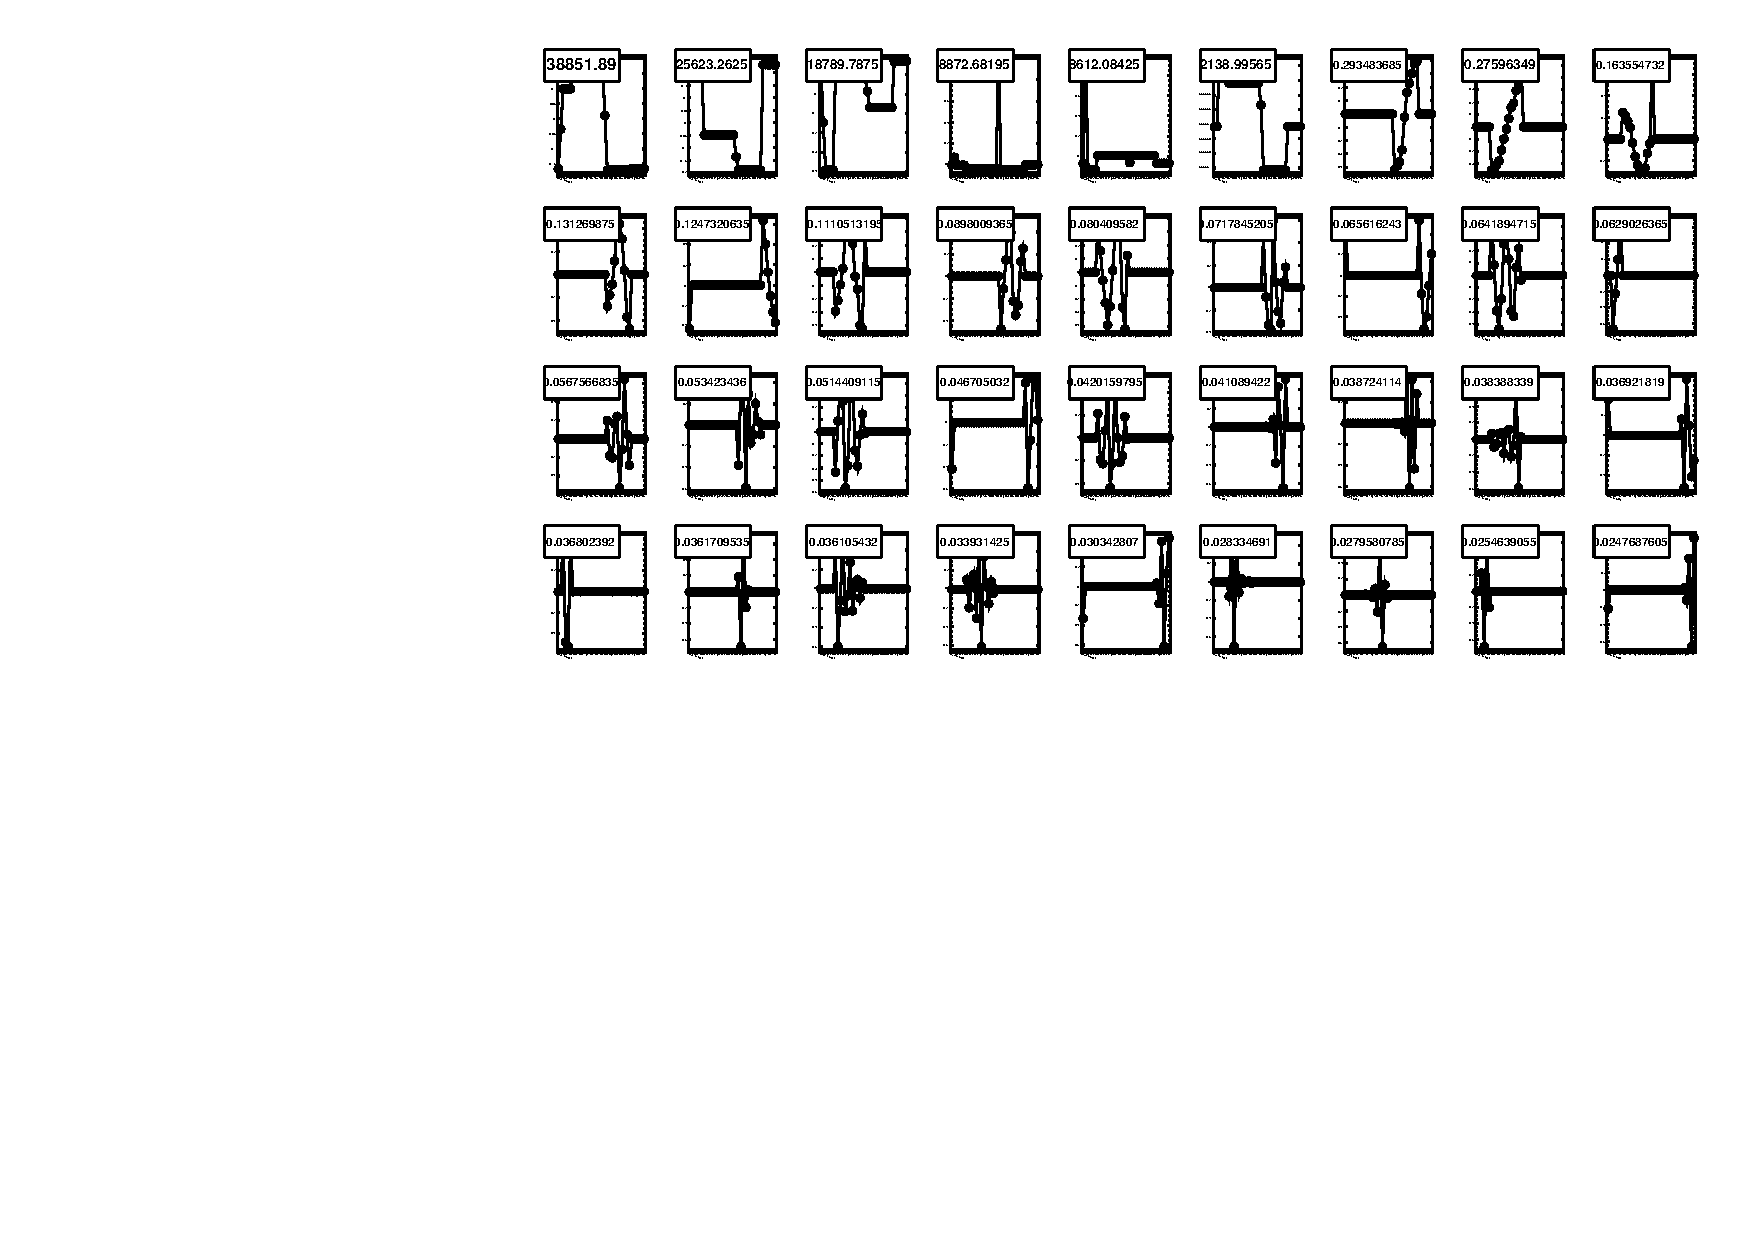
\includegraphics[width=\linewidth]{errormodes_pgnormal_p11.pdf}
\end{frame}

\begin{frame}
\frametitle{Error analysis}

\begin{columns}
\column{0.5\linewidth}

\begin{itemize}
\item Remember that ME1/1 has break-points with missing data (no PG
  and missing chambers for beam-halo)
\item These modes describe arbitrary positions of each of the sections
  relative to the others: just a reminder that we'll \mbox{need to align the sections as rigid bodies later\hspace{-5 cm}}
\end{itemize}

\column{0.5\linewidth}
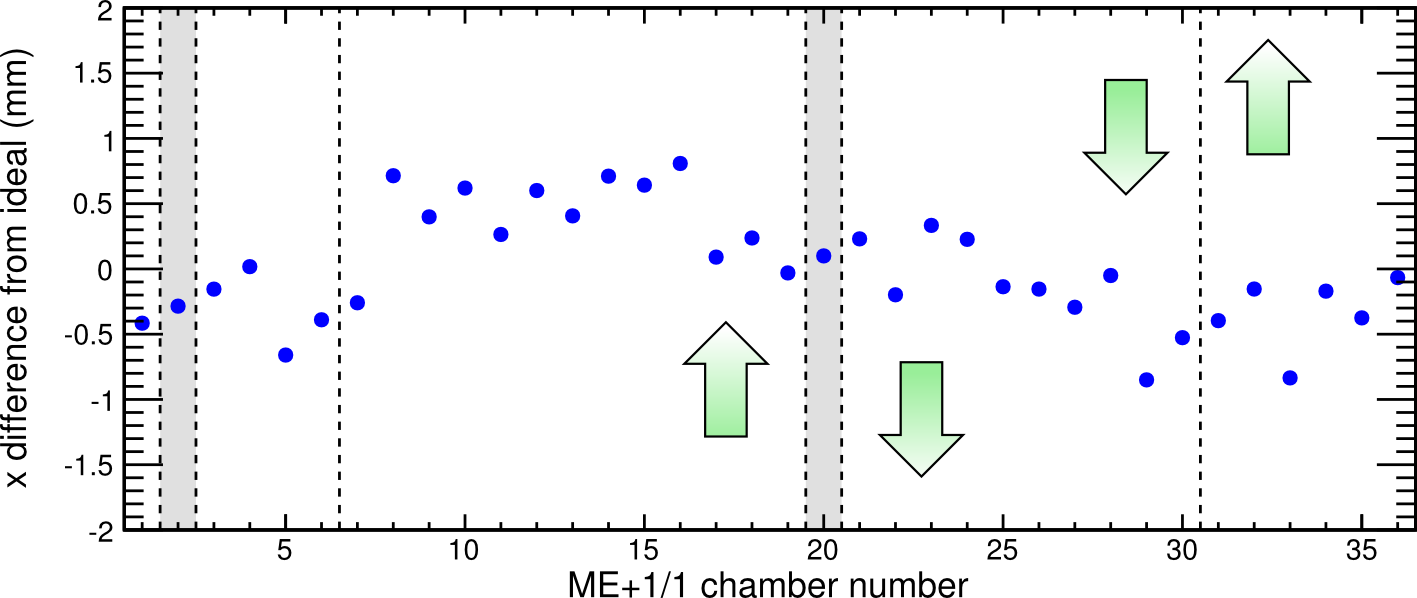
\includegraphics[width=\linewidth]{dependence_on_weights_p11.png}
\end{columns}

\vspace{0.25 cm}
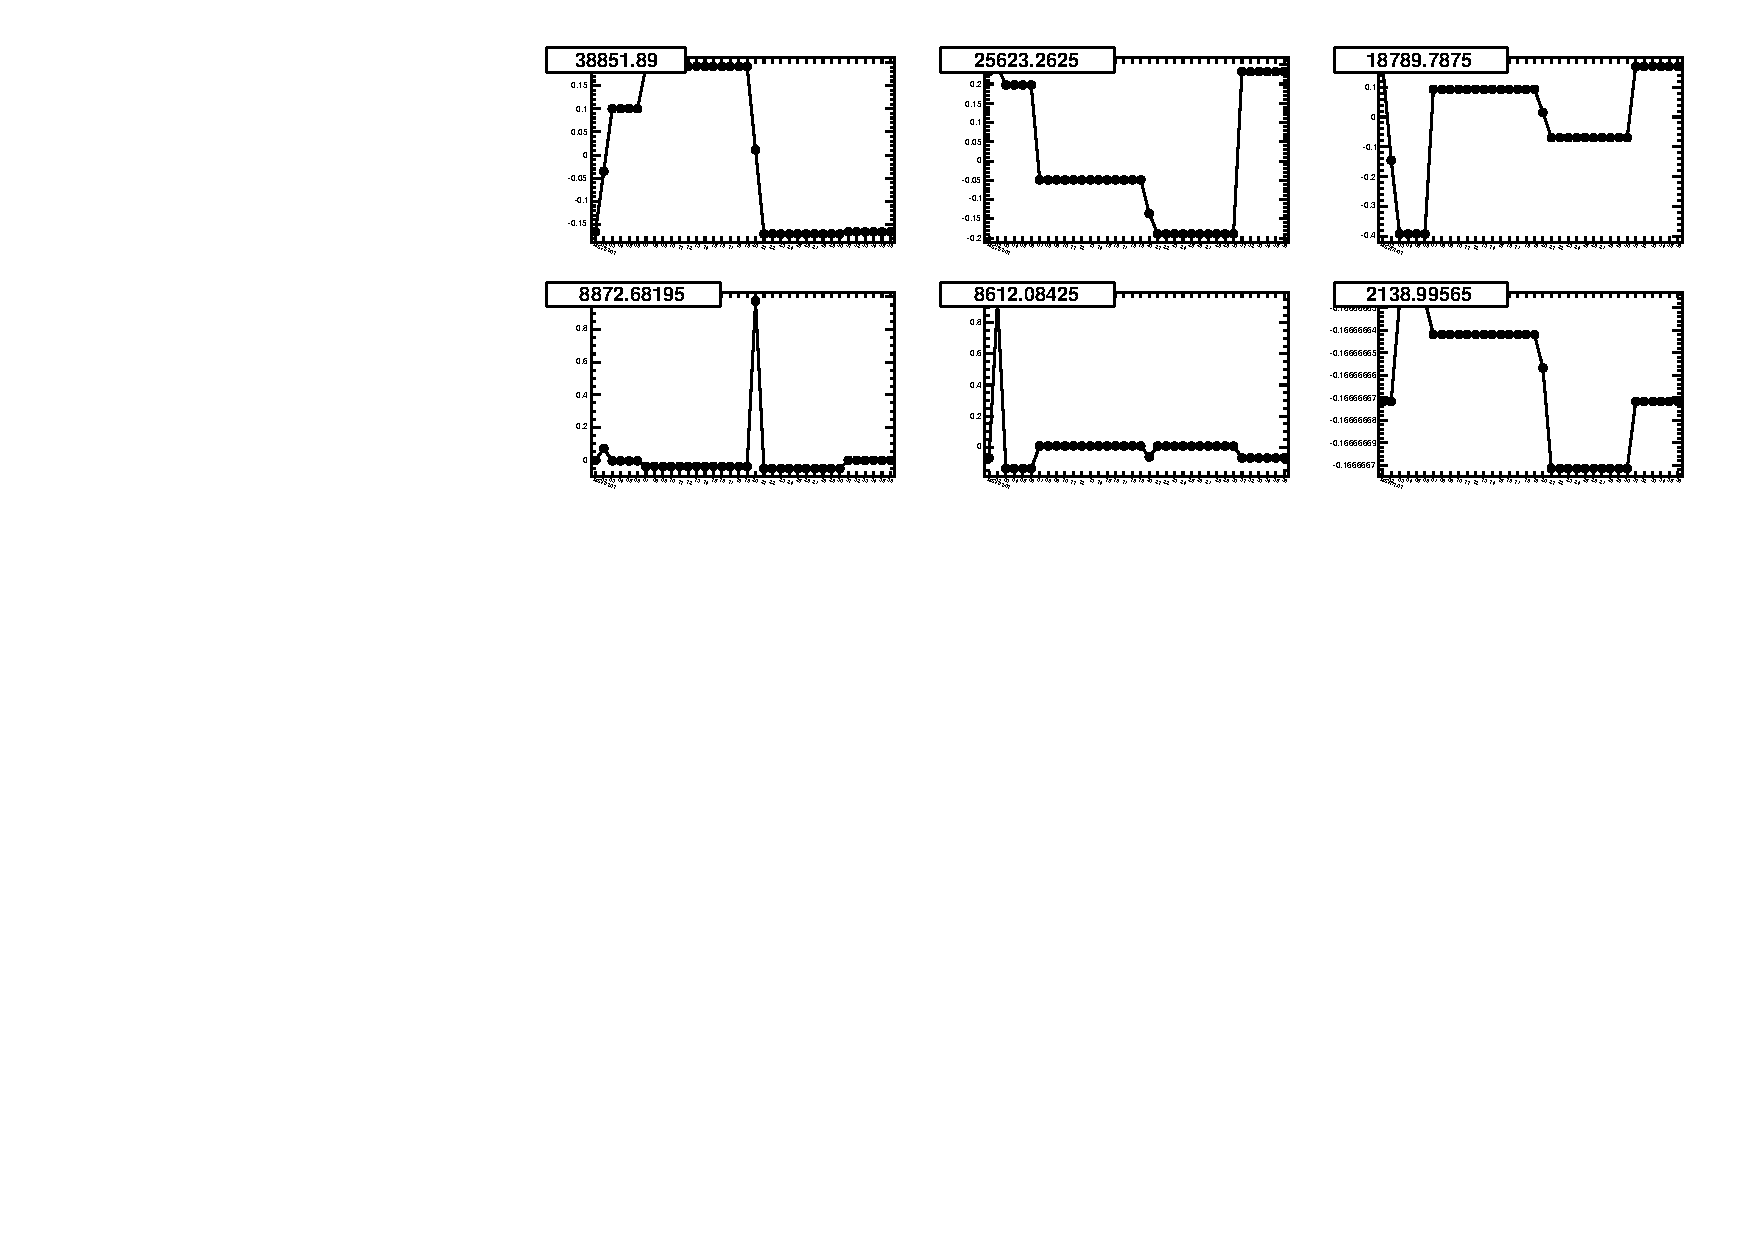
\includegraphics[width=\linewidth]{errormodes_pgnormal_p11_first6.pdf}
\end{frame}

\begin{frame}
\frametitle{Error analysis}

\begin{itemize}
\item Statistical uncertainties are in the range of a few hundred microns
\end{itemize}

\begin{center}\begin{tabular}{c c c}
\hline\hline
ring & largest mode (mm) & sum in quadrature (mm) \\\hline
ME$+$1/1 & 0.29 & 0.54 \\
ME$+$1/2 & 0.20 & 0.60 \\
ME$+$2/1 & 0.14 & 0.23 \\
ME$+$2/2 & 0.26 & 0.76 \\
ME$+$3/1 & 0.11 & 0.19 \\
ME$+$3/2 & 0.24 & 0.70 \\
ME$+$4/1 & 0.12 & 0.21 \\\hline
ME$-$1/1 & 0.47 & 0.79 \\
ME$-$1/2 & 0.15 & 0.51 \\
ME$-$2/1 & 0.13 & 0.21 \\
ME$-$2/2 & 0.15 & 0.69 \\
ME$-$3/1 & 0.09 & 0.18 \\
ME$-$3/2 & 0.19 & 0.67 \\
ME$-$4/1 & 0.10 & 0.18 \\\hline\hline
\end{tabular}\end{center}
\end{frame}

%% \section*{First section}
%% \begin{frame}
%% \begin{center}
%% \Huge \textcolor{blue}{First section}
%% \end{center}
%% \end{frame}

\begin{frame}
\frametitle{Conclusions}

\begin{itemize}\setlength{\itemsep}{0.25 cm}
\item Missing chambers forced a re-formulation of beam-halo alignment
\item Complete rings reveal that PG is still valid; use PG as a constraint
\item Need to interpret non-zero closure as radial corrections, but they form a suggestive pattern in the two endcaps
\item Beam-halo $+$ PG combination has the right limits as weight of PG constraint is varied
\item Statistical uncertainty in the result can be calculated by decomposing into modes (a few hundred microns)
\item ME1/1 ring is incomplete, only aligned in sections
\item Whole rings (and ME1/1 sections) will need to be aligned relative to the tracker with globalMuons; work on this using CRAFT-10 cosmics is underway, following same procedure as CRAFT-09
\end{itemize}

\label{numpages}
\end{frame}

\end{document}
